\documentclass[10pt,twocolumn,letterpaper]{article}
%% Welcome to Overleaf!
%% If this is your first time using LaTeX, it might be worth going through this brief presentation:
%% https://www.overleaf.com/latex/learn/free-online-introduction-to-latex-part-1

%% Researchers have been using LaTeX for decades to typeset their papers, producing beautiful, crisp documents in the process. By learning LaTeX, you are effectively following in their footsteps, and learning a highly valuable skill!

%% The \usepackage commands below can be thought of as analogous to importing libraries into Python, for instance. We've pre-formatted this for you, so you can skip right ahead to the title below.

%% Language and font encodings
\usepackage[english]{babel}
\usepackage[utf8x]{inputenc}
\usepackage[T1]{fontenc}
\usepackage{graphicx}
\usepackage{subfigure}
\usepackage{natbib}
\usepackage{listings}
\usepackage{booktabs}
\usepackage{algorithm}
\usepackage{algorithmic}
\usepackage{cuted}


%% Sets page size and margins
\usepackage[a4paper,top=3cm,bottom=2cm,left=3cm,right=3cm,marginparwidth=1.75cm]{geometry}

%% Useful packages
\usepackage{amsmath}
\usepackage[colorinlistoftodos]{todonotes}
\usepackage[colorlinks=true, allcolors=blue]{hyperref}
\usepackage{natbib}
\bibliographystyle{unsrt}

\definecolor{blve}{rgb}{0.3372549 , 0.61176471, 0.83921569}
\definecolor{gr33n}{rgb}{0.29019608, 0.7372549, 0.64705882}
\makeatletter
\lst@InstallKeywords k{class}{classstyle}\slshape{classstyle}{}ld
\makeatother
\lstset{language=C++,
	basicstyle=\ttfamily,
	keywordstyle=\color{blve}\ttfamily,
	stringstyle=\color{red}\ttfamily,
	commentstyle=\color{magenta}\ttfamily,
	morecomment=[l][\color{magenta}]{\#},
	classstyle = \bfseries\color{gr33n}, 
	tabsize=2
}
\lstset{basicstyle=\ttfamily}


%% Title
\title{
		\usefont{OT1}{bch}{b}{n}
		\normalfont \normalsize \textsc{CS121 Parallel Computing Lab 1} \\ [10pt]
		\huge Breadth First Search using OpenMP \\
}
\selectlanguage{english}
\usepackage{authblk}
\author[]{Hongtu Xu, 2019533229}
\affil[]{xuht1@shanghaitech.edu.cn}


\begin{document}
\maketitle

\begin{abstract}

In this lab, I implement two parallel BFS algorithms using OpenMP, top-down BFS and hybrid BFS \cite{beamer2012direction}. I also implement a relative fast serial algorithm and optimize the two parallel BFS algorithms using techniques like bitmap, prefix sum and so on.
\end{abstract} 

\section{Introduction}
\subsection{Compile \& Build}

All codes are tested under Ubuntu 20.04 LTS with g++ 9.3.0. You need a c++ compiler which support at least C++ 17 standard and GNU atomic compiler intrinsics and also need python3 to run bench and fetch scripts.\\
Run the benchmark by:
\begin{lstlisting}[language=bash]
make bench
\end{lstlisting}
The scripts will first fetch the four graphs from the SNAP dataset website and clone the PaRMAT \cite{wsvr} to generate three RMAT graphs. Then compile my code and finally run benchmark on these graphs automatically.

\subsection{Run}

By directly running our program, you can see the helping information. \\
There are two modes in our program, benchmark mode and running mode. \\
In benchmark mode, you need to give 6 arguments in order: input file path, the format of the input file (can be chosen from SNAP, MatrixMarket and RMAT), benchmark file output path (save the benchmark result), -1 to inform our program to run in bench mode, bfs algorithm type (can be chosen from serial, topdown and hybrid) and finally thread nums.
In running mode, you need to give 6 arguments in order: input file path, the format of the input file (can be chosen from SNAP, MatrixMarket and RMAT), output file path (save the running result), source node id, BFS algorithm type (can be chosen from serial, topdown and hybrid) and finally thread nums.

\subsection{Benchmark Configures}

I run my code on a cloud virtual machine provided by tencent cloud. The detailed information are:
\begin{table}[h]
\begin{tabular}{@{}c|c@{}}
\toprule
Config   & Value                                             \\ \midrule
CPU      & AMD EPYC $\text{ROME}^{\text{TM}}$ 7k62 (64 vCPU) \\
Memory   & 128 GB                                            \\
OS       & Ubuntu 20.04 LTS                                  \\
Kernel   & 5.4.0-77-generic                                  \\
Compiler & gcc version 9.3.0                                 \\
Optimize & -O2                                               \\ \bottomrule
\end{tabular}
\end{table}

\section{Implement Details}

\subsection{Serial Algorithm}

\begin{algorithm} 
	\caption{Serial BFS} 
	\label{sbfs} 
	\begin{algorithmic}
	    \STATE $\text{dist} \gets \{-1, -1, \cdots, -1\}$
	    \STATE $\text{parent} \gets \{-1, -1, \cdots, -1\}$
	    \STATE $\text{queue} \gets \{\text{source}\}$
	    \STATE $\text{dist[source]} \gets 0$
	    \STATE $\text{parent[source]} \gets \text{source}$
	    \WHILE{not queue.empty()}
	        \STATE $u \gets \text{queue}.\text{pop}()$
	        \FOR{$v \in \text{neighbors}(u)$}
	            \IF{$\text{dist[$v$]} = -1$}
	                \STATE $\text{dist}[v] \gets \text{dist}[u] + 1$
	                \STATE $\text{parent}[v] \gets u$
	                \STATE $\text{queue}.\text{push}(v)$
	            \ENDIF
	        \ENDFOR
	    \ENDWHILE
	\end{algorithmic} 
\end{algorithm}

In the serial algorithm, we use a queue to implement BFS. For simplicity we use std::queue to implement.\\
One observation is that we do not need to maintain a visit array, we can just use dist array to check whether a vertex is already visited. By doing this we can avoid extra memory access and due to big cache in CPU this method is faster.\\
Another optimization is the way to store the graph. I store the graph with adjacent list but implement with raw arrays, a form like CSR format for storing sparse matrix.

\subsection{Graph Storage}

As I have introduced in the serial algorithm section, I store the graph in an adjacent list with array implementation.\\
That is I store all the neighbors in a whole huge array $g$. The neighbors of the same vertex are stored consecutively. And maintain a offset array $o$ where vertex $u$'s neighbors' storage indices lie between $[o[u], o[u + 1])$. Actually, this is CSR format for storing sparse matrix.\\
Further more, from my observation, there are some unused vertices id in the graph. So, during the input process, I create a mapping to compress vertex id. This can reduce our memory cost. In the output, I just need to unmap to recover the original id.\\
Besides, also during the input process, I sort the same vertex's neighbors' id in increasing order, this can increase the probability that visiting sequence is adjacent.

\subsection{Memory Management}

I create a singleton class named MemoryManager to manage memory for big arrays. By doing this, we can simply avoid memory leak problems and reuse the memory during benchmark process, which will run bfs multiple times. The memory reuse can optimize time for memory allocation.

\subsection{Top-down Parallel BFS}

\begin{algorithm}
    \caption{Top-down step} 
	\label{topdownstep}
    \begin{algorithmic}
        \STATE \textbf{input: }vertices, frontier, next, parent, dist
        \FOR{$u \in \text{frontier}$}
            \FOR{$v \in \text{neighbors}(u)$}
                \IF{$\text{dist}[v] = -1$}
                    \STATE $\text{dist}[v] \gets \text{dist}[u] + 1, \text{parent}[v] \gets u$
                    \STATE $\text{next} \gets \text{next} \cup \{v\}$
                \ENDIF
            \ENDFOR
        \ENDFOR
    \end{algorithmic}
\end{algorithm}

\begin{algorithm}
    \caption{Top-down BFS} 
	\label{topdownstep}
    \begin{algorithmic}
        \STATE \textbf{input: }vertices, source
        \STATE $\text{frontier} \gets \{\text{source}\}$
        \STATE $\text{next} \gets \{\}$
        \STATE $\text{dist} \gets \{-1, -1, \cdots, -1\}$
        \STATE $\text{parents} \gets \{-1, -1, \cdots, -1\}$
        \STATE $\text{dist}[\text{source}] \gets 0$
        \WHILE{$\text{frontier} \neq \{\}$}
            \STATE top-down step
            \STATE $\text{frontier} \gets \text{next}$
            \STATE $\text{next} \gets \{\}$
        \ENDWHILE
    \end{algorithmic}
\end{algorithm}

To implement this in OpenMP efficiently, we need to implement bitmap and prefix sum. We can use bitmap to reduce memory traffic when checking whether a vertex is already visited. And we can use prefix sum to put neighbors into the exact position in the next frontier. See bitmap and prefix sum section for more details.\\

\begin{lstlisting}[language=C++]
while (!f->empty()) {
#pragma omp parallel for
  for (int i = 0; i < f->n; ++i)
    pi[i + 1] = deg(f->d[i]);
  prefixSumOmp(pi, f->n + 1);
  nf->n = pi[f->n];
#pragma omp parallel for schedule(guided)
  for (int i = 0; i < f->n; ++i) {
    // traverse and do topdown step
  }
  f->cullFrom(*nf, cb);
}

\end{lstlisting}

In the code above, f is the current frontier while nf is the next frontier. First we do a prefix sum on the degree array to get the next frontier's size. And by using this prefix sum array, we can put neighbors directly into the next frontier instead of using a critical section to push back one by one.\\
In the last step, we need to cull the visited vertices (duplicates) in the next frontier. Otherwise, the number of vertices in the frontier will explode. See the frontier culling section for more details.\\
Inside the top-down step, I use bit map to check whether a vertex has already been visited. This can be done through an atomic operation test-and-set. However, we can further optimize to avoid this. We first just do test operation in the bitmap, if not visited then check the dist array whether the value is $-1$ \cite{6113790,10.1145/1810479.1810534}. By doing this, we can avoid the expensive atomic operation test-and-set. In experiments, this can gain $1\% \sim 4\%$ performance improvement. The improvement is not that huge because the cost of atomic operations are much lower in modern CPUs.

\subsection{Hybrid Parallel BFS}

Instead of just using conventional top-down BFS, we can gain further optimization in some graphs by combining top-down method and bottom-up method.\\
\begin{algorithm}
    \caption{bottom-up step} 
	\label{bottomupstep}
    \begin{algorithmic}
        \STATE \textbf{input: }vertices, frontier, next, parent, dist
        \FOR{$v \in \text{vertices}$}
            \IF{$\text{dist}[v] = -1$}
                \FOR{$u \in \text{neighbors}(v)$}
                    \IF{$u \in \text{frontier}$}
                        \STATE $\text{parent}[v] \gets u$
                        \STATE $\text{dist}[v] \gets \text{dist}[u] + 1$
                        \STATE $\text{next} \gets \text{next} \cap \{v\}$
                        \STATE \textbf{break}
                    \ENDIF
                \ENDFOR
            \ENDIF
        \ENDFOR
    \end{algorithmic}
\end{algorithm}

During the parallel hybrid bfs, we maintain three variables: the number of edges to check from the frontier ($m_f$), the number of vertices in the frontier ($n_f$) and the number of edges to check from unexplored vertices ($m_u$). These metrics are easy and efficient to compute. In OpenMP, we can simply add reduction clause for these variables.\\
These variables are used to control whether we need to do top-down step or bottom-up step. We start bfs with top-down method, then when $m_f > \frac{m_u}{\alpha}$, we transfer to bottom-up method. When $n_f < \frac{n}{\beta}$, we transfer back to top-down method. We can find this hybrid parallel bfs performs better in some graphs.\\
Here, we choose $\alpha = 14$ and $\beta = 24$ follow the best parameter described in the paper \cite{beamer2012direction}.\\

\subsection{Bit Map}

Store size of int32 or int64 times 8 bool into one int. In C++, we can use a template class to easily switch between int32 and int64. The test and set operation of bitmap is easy to implement by just taking some bit operations.\\
An important one is test-and-set operation, here I use GNU compiler intrinsics:
\begin{lstlisting}[language=C++]
__atomic_fetch_or(&d[index], 
    bitOffset, __ATOMIC_SEQ_CST);
\end{lstlisting}
This is an atomic intrinsics operation provided by gcc, which is relatively fast. Actually, as I have discussed in top-down bfs section, we can avoid this to gain a better performance.

\subsection{Prefix Sum in OpenMP}

\begin{lstlisting}[language=C++]
#pragma omp parallel
{
  int id = omp_get_thread_num();
  T s = 0;
#pragma omp for schedule(static)\
    nowait
  for (int i = 0; i < n; ++i) {
    s += a[i];
    a[i] = s;
  }
  buffer[id + 1] = s;

#pragma omp barrier
  T offset = 0;
  for (int i = 1; i < id + 1; ++i) 
    offset += buffer[i];
#pragma omp for schedule(static)
  for (std::uint32_t i = 0; i < n; ++i) 
    a[i] += offset;
}
\end{lstlisting}

First, we use different threads to prefix sum the numbers distributed to them locally. Then, store each thread's sum into a buffer, get the prefix sum in the buffer of the threads whose thread id is less than or equal to the current thread, then add the sum into each number it owns.

\subsection{Frontier Culling}

We need to cull the next frontier to avoid vertices explosion. This is a filter process, first we write into a buffer: $0$ for this item should be filtered and $1$ for this item should be preserved. Then we apply prefix sum on this buffer, after that, we can directly write preserved items into the correct position.

\subsection{IO Optimization}

Since we need to do a lot of experiments, we need to run bfs with 20 random sources and this should be run multiple times to reduce uncertainty and we need to run benchmark with number of threads from $1$ to $64$. In addition, the IO takes a very high percentage of the total running time.\\
In order to run experiments faster, we need to optimize the IO. As I introduced in the run code section, you need to pass the input file's format. This format is used in the IO optimization, my code can directly load graphs from SNAP and RMAT format. No need to convert it to MatrixMarket format.\\
While reading, I maintain a buffered reader, that is I create a large buffer, each time I use std::fread to read a large block of the file into the memory, then parse the the numbers manually, which is much faster than fscanf or fstream (more than 20 times faster).\\
By doing this, the first four graph all can be loaded (including pre-processings like id mapping construction) in 5 second and the RMAT can also be loaded in 1min.

\section{Results}

After running experiments, the benmark result is listed as follows:

\begin{strip}
\centering
\begin{tabular}{@{}c|ccccccc@{}}
\toprule
Graph            & Single Thread  & Topdown, threads     & Hybrid, threads      & Speedup & Time (s) & StdDev \\ \midrule
web-Stanford     & 227.185 & 675.243, 4  & 648.741, 5  & 2.972 & 0.00342469 & 1.38624    \\
roadNet-CA       & 63.536  & 208.959, 4  & 204.252, 4  & 3.289  & 0.0274864 & 0.552123 \\
com-Orkut        & 373.057 & \textbf{5291.94, 64} & 5280.75, 64 & 14.185 & 0.0225889 & 99.7608 \\
soc-Livejournal1 & 72.3957 & 1439.49, 63 & 1439.56, 63 & 19.885 & 0.047927 & 15.9759 \\
RMAT1            & 18.965 & 559.64, 63  & 549.926, 64 & \textbf{29.526} & 1.78583 & 6.17689  \\
RMAT2            & 33.6309 &    906.489, 64         &   912.044, 64          &   27.119 & 1.09644 & 11.5889      \\
RMAT3            &    138.81     & 2293.06, 62            & 2307.07, 63            &16.620 & 0.43345 & 1000.97         \\ \bottomrule
\end{tabular}

\end{strip}

The performance are measured in MTEPS (millions of edges traversed per second), the baseline is the conventional top-down with single thread. We can find that the hybrid method only performs a little better in some graphs, it cannot significantly increase the peak performance. However, in the experiments, I find that the hybrid method can perform better in many thread nums.\\
In the first two graphs, our peak speedup is around $3$, I think this is because the average degree of the graph is not much enough and the graph is also much smaller than the rest, we reach the peak performance using just $4$ threads.\\
In the third graph, com-Orkut, our algorithm reach the peak performance of $5291.94$ MTEPS, which is very efficient. And in the experiment, our performance is always increasing as the number of threads increase.\\
In the soc-Livejournal1 graph, we also obtain a relatively good speedup.\\
For the three big random graph, the absolute performance in MTEPS is not that high because of memory access, these graph need too much memory and the cache performance is not that good. However, our algorithm gains a very good speedup in these graphs. The performance almost always increases as the number of threads increase.\\
And in these graphs, we reach our peak speedup of $29.526$, which is good enough and our algorithm is efficient.

\begin{strip}
    \centering
    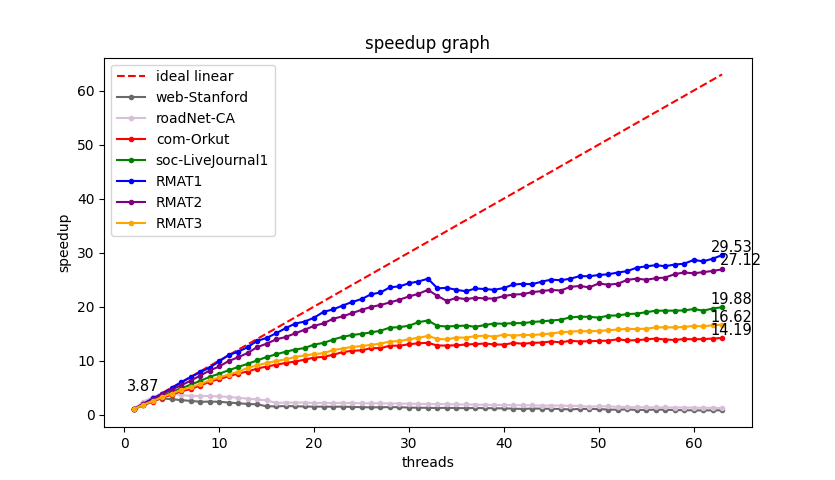
\includegraphics[scale=0.8]{figures/speedup.png}
\end{strip}

\newpage

\bibliography{bibliography}

\section{Appendix}

All the experiment data are listed on the next page.

\newpage

\begin{table}[h]
\renewcommand\arraystretch{0.8}
\centering
\begin{tabular}{@{}c|ccc@{}}
\toprule
Threads          & MTEPS  & StdDev     & Time (s)      \\ \midrule
1 & 227.185 & 1.496 & 0.010179 \\
2 & 433.386 & 1.517 & 0.005336 \\
3 & 543.152 & 1.443 & 0.004258 \\
4 & 675.243 & 1.386 & 0.003425 \\
5 & 622.034 & 1.349 & 0.003718 \\
6 & 593.315 & 1.319 & 0.003898 \\
7 & 575.647 & 1.315 & 0.004017 \\
8 & 539.476 & 1.412 & 0.004287 \\
9 & 517.574 & 1.336 & 0.004468 \\
10 & 536.526 & 1.307 & 0.004310 \\
11 & 495.762 & 1.335 & 0.004665 \\
12 & 427.408 & 1.769 & 0.005411 \\
13 & 445.938 & 1.365 & 0.005186 \\
14 & 410.805 & 1.385 & 0.005629 \\
15 & 345.527 & 1.452 & 0.006693 \\
16 & 338.506 & 1.467 & 0.006831 \\
17 & 357.785 & 1.448 & 0.006463 \\
18 & 347.207 & 1.465 & 0.006660 \\
19 & 340.809 & 1.511 & 0.006785 \\
20 & 323.520 & 1.554 & 0.007148 \\
21 & 334.867 & 1.502 & 0.006906 \\
22 & 319.326 & 1.545 & 0.007242 \\
23 & 333.096 & 1.563 & 0.006942 \\
24 & 319.401 & 1.542 & 0.007240 \\
25 & 300.344 & 1.577 & 0.007699 \\
26 & 291.765 & 1.583 & 0.007926 \\
27 & 306.569 & 1.576 & 0.007543 \\
28 & 303.731 & 1.606 & 0.007614 \\
29 & 309.752 & 1.544 & 0.007466 \\
30 & 293.676 & 1.546 & 0.007874 \\
31 & 288.308 & 1.623 & 0.008021 \\
32 & 280.844 & 1.577 & 0.008234 \\
33 & 267.614 & 1.603 & 0.008641 \\
34 & 251.999 & 1.622 & 0.009177 \\
35 & 267.411 & 1.665 & 0.008648 \\
36 & 269.803 & 1.592 & 0.008571 \\
37 & 247.019 & 1.617 & 0.009362 \\
38 & 270.403 & 1.579 & 0.008552 \\
39 & 266.204 & 1.570 & 0.008687 \\
40 & 259.412 & 1.587 & 0.008914 \\
41 & 249.951 & 1.663 & 0.009252 \\
42 & 234.790 & 1.652 & 0.009849 \\
43 & 255.117 & 1.624 & 0.009064 \\
44 & 247.736 & 1.585 & 0.009335 \\
45 & 243.743 & 1.596 & 0.009487 \\
46 & 231.102 & 1.621 & 0.010006 \\
47 & 216.896 & 1.691 & 0.010662 \\
48 & 236.481 & 1.596 & 0.009779 \\
49 & 234.245 & 1.647 & 0.009872 \\
50 & 230.345 & 1.610 & 0.010039 \\
51 & 196.082 & 1.632 & 0.011794 \\
52 & 202.631 & 1.676 & 0.011412 \\
53 & 200.286 & 1.648 & 0.011546 \\
54 & 193.876 & 1.688 & 0.011928 \\
55 & 196.090 & 1.662 & 0.011793 \\
56 & 208.272 & 1.659 & 0.011103 \\
57 & 178.018 & 1.686 & 0.012990 \\
58 & 189.542 & 1.679 & 0.012200 \\
59 & 183.522 & 1.652 & 0.012601 \\
60 & 175.918 & 1.721 & 0.013145 \\
61 & 174.028 & 1.711 & 0.013288 \\
62 & 177.212 & 1.658 & 0.013049 \\
63 & 177.172 & 1.678 & 0.013052 \\
64 & 166.524 & 1.705 & 0.013887 \\
\bottomrule
\end{tabular}
\caption{web-Stanford top-down}
\end{table}
\begin{table}[h]
\renewcommand\arraystretch{0.8}
\centering
\begin{tabular}{@{}c|ccc@{}}
\toprule
Threads          & MTEPS  & StdDev     & Time (s)      \\ \midrule
1 & 227.937 & 1.492 & 0.010145 \\
2 & 490.973 & 1.428 & 0.004710 \\
3 & 603.280 & 1.427 & 0.003833 \\
4 & 605.104 & 1.412 & 0.003822 \\
5 & 648.741 & 1.348 & 0.003565 \\
6 & 607.349 & 1.355 & 0.003808 \\
7 & 573.509 & 1.312 & 0.004032 \\
8 & 539.257 & 1.293 & 0.004288 \\
9 & 543.633 & 1.298 & 0.004254 \\
10 & 539.715 & 1.322 & 0.004285 \\
11 & 505.165 & 1.331 & 0.004578 \\
12 & 476.320 & 1.352 & 0.004855 \\
13 & 433.943 & 1.759 & 0.005329 \\
14 & 430.489 & 1.545 & 0.005372 \\
15 & 349.422 & 1.559 & 0.006618 \\
16 & 345.103 & 1.461 & 0.006701 \\
17 & 359.240 & 1.484 & 0.006437 \\
18 & 350.233 & 1.486 & 0.006603 \\
19 & 334.184 & 1.516 & 0.006920 \\
20 & 331.572 & 1.518 & 0.006974 \\
21 & 332.425 & 1.486 & 0.006956 \\
22 & 328.930 & 1.564 & 0.007030 \\
23 & 315.951 & 1.558 & 0.007319 \\
24 & 320.247 & 1.589 & 0.007221 \\
25 & 310.767 & 1.557 & 0.007441 \\
26 & 303.474 & 1.583 & 0.007620 \\
27 & 302.316 & 1.575 & 0.007649 \\
28 & 313.654 & 1.596 & 0.007373 \\
29 & 296.558 & 1.606 & 0.007798 \\
30 & 289.216 & 1.607 & 0.007996 \\
31 & 283.593 & 1.615 & 0.008154 \\
32 & 283.091 & 1.598 & 0.008169 \\
33 & 274.701 & 1.640 & 0.008418 \\
34 & 285.365 & 1.630 & 0.008104 \\
35 & 271.899 & 1.591 & 0.008505 \\
36 & 249.157 & 1.596 & 0.009281 \\
37 & 275.492 & 1.618 & 0.008394 \\
38 & 264.243 & 1.610 & 0.008751 \\
39 & 252.926 & 1.572 & 0.009143 \\
40 & 255.612 & 1.635 & 0.009047 \\
41 & 232.081 & 1.626 & 0.009964 \\
42 & 237.053 & 1.619 & 0.009755 \\
43 & 242.901 & 1.579 & 0.009520 \\
44 & 235.143 & 1.613 & 0.009834 \\
45 & 232.968 & 1.650 & 0.009926 \\
46 & 234.023 & 1.667 & 0.009881 \\
47 & 211.662 & 1.652 & 0.010925 \\
48 & 226.766 & 1.678 & 0.010198 \\
49 & 220.611 & 1.627 & 0.010482 \\
50 & 213.731 & 1.684 & 0.010820 \\
51 & 211.508 & 1.644 & 0.010933 \\
52 & 194.382 & 1.662 & 0.011897 \\
53 & 218.737 & 1.677 & 0.010572 \\
54 & 190.824 & 1.733 & 0.012119 \\
55 & 198.547 & 1.658 & 0.011647 \\
56 & 191.752 & 1.662 & 0.012060 \\
57 & 205.727 & 1.659 & 0.011241 \\
58 & 177.468 & 1.644 & 0.013031 \\
59 & 178.307 & 1.669 & 0.012969 \\
60 & 173.671 & 1.610 & 0.013315 \\
61 & 175.288 & 1.697 & 0.013193 \\
62 & 177.268 & 1.674 & 0.013045 \\
63 & 173.180 & 1.692 & 0.013353 \\
64 & 168.822 & 1.683 & 0.013698 \\
\bottomrule
\end{tabular}
\caption{web-Stanford hybrid}
\end{table}
\begin{table}[h]
\renewcommand\arraystretch{0.8}
\centering
\begin{tabular}{@{}c|ccc@{}}
\toprule
Threads          & MTEPS  & StdDev     & Time (s)      \\ \midrule
1 & 63.536 & 0.046 & 0.087087 \\
2 & 126.437 & 0.409 & 0.043763 \\
3 & 170.751 & 0.390 & 0.032405 \\
4 & 201.307 & 0.552 & 0.027486 \\
5 & 208.959 & 0.384 & 0.026480 \\
6 & 194.068 & 0.391 & 0.028512 \\
7 & 187.587 & 0.476 & 0.029497 \\
8 & 185.714 & 0.338 & 0.029794 \\
9 & 184.917 & 0.368 & 0.029923 \\
10 & 180.929 & 0.602 & 0.030582 \\
11 & 176.582 & 0.425 & 0.031335 \\
12 & 167.351 & 0.364 & 0.033064 \\
13 & 159.158 & 0.667 & 0.034766 \\
14 & 150.570 & 0.569 & 0.036749 \\
15 & 132.198 & 1.517 & 0.041856 \\
16 & 115.717 & 0.453 & 0.047817 \\
17 & 119.304 & 0.464 & 0.046379 \\
18 & 118.957 & 0.483 & 0.046514 \\
19 & 120.476 & 0.558 & 0.045928 \\
20 & 115.477 & 0.538 & 0.047916 \\
21 & 116.835 & 0.488 & 0.047359 \\
22 & 114.730 & 0.556 & 0.048228 \\
23 & 117.491 & 0.518 & 0.047095 \\
24 & 115.521 & 0.567 & 0.047898 \\
25 & 111.179 & 0.546 & 0.049768 \\
26 & 111.659 & 0.539 & 0.049554 \\
27 & 113.130 & 0.548 & 0.048910 \\
28 & 110.632 & 0.543 & 0.050015 \\
29 & 110.502 & 0.555 & 0.050073 \\
30 & 107.941 & 0.579 & 0.051261 \\
31 & 106.466 & 0.547 & 0.051972 \\
32 & 105.837 & 0.566 & 0.052281 \\
33 & 104.126 & 0.551 & 0.053140 \\
34 & 104.394 & 0.578 & 0.053003 \\
35 & 101.750 & 0.572 & 0.054381 \\
36 & 100.766 & 0.597 & 0.054911 \\
37 & 99.318 & 0.623 & 0.055712 \\
38 & 97.549 & 0.603 & 0.056723 \\
39 & 97.685 & 0.609 & 0.056643 \\
40 & 94.682 & 0.553 & 0.058440 \\
41 & 93.789 & 0.573 & 0.058997 \\
42 & 93.690 & 0.624 & 0.059059 \\
43 & 90.454 & 0.605 & 0.061171 \\
44 & 89.147 & 0.575 & 0.062068 \\
45 & 86.353 & 0.592 & 0.064077 \\
46 & 88.771 & 0.627 & 0.062331 \\
47 & 85.654 & 0.551 & 0.064600 \\
48 & 87.244 & 0.599 & 0.063423 \\
49 & 76.117 & 0.557 & 0.072693 \\
50 & 83.374 & 0.589 & 0.066366 \\
51 & 76.310 & 0.556 & 0.072510 \\
52 & 76.364 & 0.588 & 0.072458 \\
53 & 75.438 & 0.585 & 0.073348 \\
54 & 72.748 & 0.573 & 0.076061 \\
55 & 70.582 & 0.583 & 0.078394 \\
56 & 67.867 & 0.582 & 0.081530 \\
57 & 71.462 & 0.591 & 0.077429 \\
58 & 70.448 & 0.580 & 0.078543 \\
59 & 70.590 & 0.651 & 0.078385 \\
60 & 68.157 & 0.594 & 0.081183 \\
61 & 67.993 & 0.630 & 0.081379 \\
62 & 67.695 & 0.661 & 0.081737 \\
63 & 65.103 & 0.731 & 0.084991 \\
64 & 61.135 & 0.737 & 0.090509 \\
\bottomrule
\end{tabular}
\caption{roadNet-CA top-down}
\end{table}
\begin{table}[h]
\renewcommand\arraystretch{0.8}
\centering
\begin{tabular}{@{}c|ccc@{}}
\toprule
Threads          & MTEPS  & StdDev     & Time (s)      \\ \midrule
1 & 64.990 & 0.065 & 0.085139 \\
2 & 129.330 & 0.248 & 0.042784 \\
3 & 177.361 & 0.269 & 0.031197 \\
4 & 204.252 & 0.387 & 0.027090 \\
5 & 203.879 & 0.570 & 0.027140 \\
6 & 193.994 & 0.385 & 0.028523 \\
7 & 187.655 & 0.330 & 0.029486 \\
8 & 185.081 & 0.317 & 0.029896 \\
9 & 183.330 & 0.523 & 0.030182 \\
10 & 178.658 & 0.343 & 0.030971 \\
11 & 177.387 & 0.406 & 0.031193 \\
12 & 166.612 & 0.387 & 0.033210 \\
13 & 159.637 & 0.405 & 0.034661 \\
14 & 151.499 & 0.751 & 0.036523 \\
15 & 141.900 & 0.586 & 0.038994 \\
16 & 117.185 & 0.460 & 0.047218 \\
17 & 120.118 & 0.483 & 0.046065 \\
18 & 120.118 & 0.490 & 0.046065 \\
19 & 120.418 & 0.444 & 0.045950 \\
20 & 114.444 & 0.537 & 0.048349 \\
21 & 114.521 & 0.552 & 0.048316 \\
22 & 114.788 & 0.496 & 0.048204 \\
23 & 116.727 & 0.521 & 0.047403 \\
24 & 114.623 & 0.509 & 0.048273 \\
25 & 112.818 & 0.528 & 0.049045 \\
26 & 112.871 & 0.526 & 0.049022 \\
27 & 111.180 & 0.536 & 0.049768 \\
28 & 109.971 & 0.512 & 0.050315 \\
29 & 107.616 & 0.564 & 0.051416 \\
30 & 104.108 & 0.638 & 0.053149 \\
31 & 106.876 & 0.566 & 0.051772 \\
32 & 104.293 & 0.588 & 0.053054 \\
33 & 101.115 & 0.601 & 0.054722 \\
34 & 103.115 & 0.568 & 0.053660 \\
35 & 99.106 & 0.641 & 0.055831 \\
36 & 100.189 & 0.618 & 0.055228 \\
37 & 99.843 & 0.608 & 0.055419 \\
38 & 94.562 & 0.588 & 0.058514 \\
39 & 90.153 & 0.678 & 0.061376 \\
40 & 93.856 & 0.583 & 0.058955 \\
41 & 92.654 & 0.588 & 0.059719 \\
42 & 86.854 & 0.539 & 0.063707 \\
43 & 92.202 & 0.591 & 0.060012 \\
44 & 89.118 & 0.686 & 0.062089 \\
45 & 90.448 & 0.523 & 0.061176 \\
46 & 89.653 & 0.558 & 0.061718 \\
47 & 87.035 & 0.610 & 0.063575 \\
48 & 77.941 & 0.709 & 0.070993 \\
49 & 78.048 & 0.548 & 0.070895 \\
50 & 74.819 & 0.575 & 0.073955 \\
51 & 81.592 & 0.668 & 0.067816 \\
52 & 76.831 & 0.720 & 0.072018 \\
53 & 75.117 & 0.595 & 0.073661 \\
54 & 73.212 & 0.595 & 0.075578 \\
55 & 73.619 & 0.612 & 0.075161 \\
56 & 70.787 & 0.636 & 0.078166 \\
57 & 70.447 & 0.602 & 0.078545 \\
58 & 69.615 & 0.605 & 0.079483 \\
59 & 69.074 & 0.567 & 0.080105 \\
60 & 68.695 & 0.744 & 0.080548 \\
61 & 67.393 & 0.585 & 0.082103 \\
62 & 67.668 & 0.619 & 0.081771 \\
63 & 65.222 & 0.642 & 0.084837 \\
64 & 63.638 & 0.714 & 0.086949 \\
\bottomrule
\end{tabular}
\caption{roadNet-CA hybrid}
\end{table}
\begin{table}[h]
\renewcommand\arraystretch{0.8}
\centering
\begin{tabular}{@{}c|ccc@{}}
\toprule
Threads          & MTEPS  & StdDev     & Time (s)      \\ \midrule
1 & 374.800 & 117.463 & 0.312660 \\
2 & 624.144 & 109.925 & 0.187753 \\
3 & 860.299 & 108.191 & 0.136214 \\
4 & 1165.000 & 108.844 & 0.100588 \\
5 & 1379.340 & 108.573 & 0.084957 \\
6 & 1558.860 & 105.412 & 0.075173 \\
7 & 1762.510 & 106.749 & 0.066488 \\
8 & 1988.230 & 106.858 & 0.058939 \\
9 & 2271.510 & 108.503 & 0.051589 \\
10 & 2424.630 & 108.177 & 0.048331 \\
11 & 2623.320 & 109.033 & 0.044671 \\
12 & 2835.580 & 108.332 & 0.041327 \\
13 & 2958.730 & 108.960 & 0.039607 \\
14 & 3178.190 & 108.092 & 0.036872 \\
15 & 3297.570 & 108.338 & 0.035537 \\
16 & 3415.700 & 108.912 & 0.034308 \\
17 & 3563.230 & 109.133 & 0.032887 \\
18 & 3654.710 & 110.269 & 0.032064 \\
19 & 3760.860 & 109.977 & 0.031159 \\
20 & 3937.910 & 110.243 & 0.029758 \\
21 & 3986.240 & 110.746 & 0.029397 \\
22 & 4130.730 & 109.232 & 0.028369 \\
23 & 4314.060 & 109.433 & 0.027164 \\
24 & 4392.380 & 108.789 & 0.026679 \\
25 & 4425.170 & 109.782 & 0.026482 \\
26 & 4502.310 & 109.851 & 0.026028 \\
27 & 4585.530 & 108.050 & 0.025555 \\
28 & 4759.110 & 109.216 & 0.024623 \\
29 & 4757.550 & 109.650 & 0.024631 \\
30 & 4816.790 & 109.150 & 0.024328 \\
31 & 4872.720 & 108.502 & 0.024049 \\
32 & 4853.710 & 108.059 & 0.024143 \\
33 & 4756.910 & 107.608 & 0.024635 \\
34 & 4769.110 & 108.101 & 0.024572 \\
35 & 4788.540 & 107.560 & 0.024472 \\
36 & 4841.110 & 106.958 & 0.024206 \\
37 & 4872.620 & 107.060 & 0.024050 \\
38 & 4905.430 & 107.290 & 0.023889 \\
39 & 4822.300 & 106.460 & 0.024301 \\
40 & 4820.570 & 106.199 & 0.024309 \\
41 & 4951.120 & 105.491 & 0.023668 \\
42 & 4893.700 & 104.647 & 0.023946 \\
43 & 4935.560 & 105.384 & 0.023743 \\
44 & 4978.230 & 105.226 & 0.023540 \\
45 & 5046.930 & 105.418 & 0.023219 \\
46 & 4989.740 & 103.508 & 0.023485 \\
47 & 5026.400 & 103.785 & 0.023314 \\
48 & 5047.380 & 103.994 & 0.023217 \\
49 & 5000.770 & 104.425 & 0.023433 \\
50 & 5090.570 & 103.988 & 0.023020 \\
51 & 5103.990 & 104.108 & 0.022960 \\
52 & 5174.240 & 104.239 & 0.022648 \\
53 & 5121.430 & 102.051 & 0.022881 \\
54 & 5101.020 & 102.773 & 0.022973 \\
55 & 5136.910 & 102.116 & 0.022812 \\
56 & 5235.040 & 101.863 & 0.022385 \\
57 & 5148.830 & 100.991 & 0.022759 \\
58 & 5154.040 & 102.371 & 0.022737 \\
59 & 5220.430 & 101.220 & 0.022447 \\
60 & 5138.460 & 100.481 & 0.022805 \\
61 & 5213.890 & 100.581 & 0.022476 \\
62 & 5250.480 & 99.694 & 0.022319 \\
63 & 5291.940 & 98.893 & 0.022144 \\
64 & 5258.370 & 98.453 & 0.022285 \\
\bottomrule
\end{tabular}
\caption{com-Orkut top-down}
\end{table}
\begin{table}[h]
\renewcommand\arraystretch{0.8}
\centering
\begin{tabular}{@{}c|ccc@{}}
\toprule
Threads          & MTEPS  & StdDev     & Time (s)      \\ \midrule
1 & 373.057 & 117.513 & 0.314121 \\
2 & 643.040 & 110.912 & 0.182236 \\
3 & 896.053 & 108.606 & 0.130779 \\
4 & 1067.720 & 107.202 & 0.109752 \\
5 & 1346.180 & 106.567 & 0.087050 \\
6 & 1609.290 & 107.719 & 0.072818 \\
7 & 1756.340 & 106.820 & 0.066721 \\
8 & 2005.570 & 106.501 & 0.058430 \\
9 & 2259.890 & 108.304 & 0.051854 \\
10 & 2459.030 & 109.469 & 0.047655 \\
11 & 2639.670 & 109.408 & 0.044394 \\
12 & 2832.200 & 108.073 & 0.041376 \\
13 & 2974.360 & 109.310 & 0.039398 \\
14 & 3158.630 & 108.457 & 0.037100 \\
15 & 3318.720 & 108.553 & 0.035310 \\
16 & 3445.430 & 108.648 & 0.034012 \\
17 & 3553.300 & 109.027 & 0.032979 \\
18 & 3662.370 & 110.160 & 0.031997 \\
19 & 3793.170 & 109.977 & 0.030894 \\
20 & 3927.410 & 109.470 & 0.029838 \\
21 & 3952.410 & 110.598 & 0.029649 \\
22 & 4130.880 & 109.023 & 0.028368 \\
23 & 4295.710 & 109.243 & 0.027280 \\
24 & 4406.520 & 109.347 & 0.026594 \\
25 & 4436.700 & 109.910 & 0.026413 \\
26 & 4590.460 & 109.079 & 0.025528 \\
27 & 4585.830 & 108.080 & 0.025554 \\
28 & 4719.230 & 108.332 & 0.024831 \\
29 & 4752.230 & 109.671 & 0.024659 \\
30 & 4856.510 & 109.731 & 0.024130 \\
31 & 4926.870 & 108.206 & 0.023785 \\
32 & 4954.900 & 108.028 & 0.023650 \\
33 & 4770.440 & 108.613 & 0.024565 \\
34 & 4661.500 & 107.291 & 0.025139 \\
35 & 4772.790 & 107.291 & 0.024553 \\
36 & 4801.180 & 107.379 & 0.024408 \\
37 & 4866.380 & 106.407 & 0.024081 \\
38 & 4855.870 & 105.745 & 0.024133 \\
39 & 4849.410 & 105.416 & 0.024165 \\
40 & 4832.190 & 106.005 & 0.024251 \\
41 & 4816.090 & 105.328 & 0.024332 \\
42 & 4893.360 & 103.893 & 0.023948 \\
43 & 4950.030 & 105.676 & 0.023674 \\
44 & 4974.720 & 104.904 & 0.023556 \\
45 & 4996.050 & 105.678 & 0.023456 \\
46 & 4932.660 & 105.349 & 0.023757 \\
47 & 5101.800 & 104.638 & 0.022969 \\
48 & 4976.920 & 102.979 & 0.023546 \\
49 & 5069.300 & 104.111 & 0.023117 \\
50 & 5074.080 & 101.990 & 0.023095 \\
51 & 5061.060 & 102.483 & 0.023154 \\
52 & 5199.960 & 102.921 & 0.022536 \\
53 & 5091.570 & 102.244 & 0.023016 \\
54 & 5138.630 & 102.851 & 0.022805 \\
55 & 5190.800 & 101.316 & 0.022575 \\
56 & 5252.690 & 102.899 & 0.022309 \\
57 & 5183.050 & 101.218 & 0.022609 \\
58 & 5022.790 & 100.109 & 0.023331 \\
59 & 5181.450 & 101.077 & 0.022616 \\
60 & 5197.900 & 100.415 & 0.022545 \\
61 & 5175.880 & 99.762 & 0.022641 \\
62 & 5206.630 & 99.302 & 0.022507 \\
63 & 5187.730 & 99.761 & 0.022589 \\
64 & 5280.750 & 99.110 & 0.022191 \\
\bottomrule
\end{tabular}
\caption{com-Orkut hybrid}
\end{table}
\begin{table}[h]
\renewcommand\arraystretch{0.8}
\centering
\begin{tabular}{@{}c|ccc@{}}
\toprule
Threads          & MTEPS  & StdDev     & Time (s)      \\ \midrule
1 & 73.368 & 15.860 & 0.940379 \\
2 & 129.099 & 15.884 & 0.534426 \\
3 & 189.150 & 15.907 & 0.364756 \\
4 & 237.009 & 15.928 & 0.291102 \\
5 & 294.273 & 15.936 & 0.234455 \\
6 & 350.570 & 15.927 & 0.196805 \\
7 & 401.378 & 15.956 & 0.171892 \\
8 & 450.747 & 15.950 & 0.153065 \\
9 & 505.560 & 15.926 & 0.136470 \\
10 & 547.939 & 15.944 & 0.125915 \\
11 & 593.313 & 15.921 & 0.116286 \\
12 & 638.654 & 15.927 & 0.108030 \\
13 & 669.242 & 15.947 & 0.103092 \\
14 & 725.609 & 15.924 & 0.095084 \\
15 & 771.965 & 15.955 & 0.089374 \\
16 & 806.785 & 15.954 & 0.085517 \\
17 & 842.310 & 15.960 & 0.081910 \\
18 & 871.806 & 15.955 & 0.079139 \\
19 & 889.950 & 15.978 & 0.077525 \\
20 & 929.610 & 15.948 & 0.074218 \\
21 & 960.994 & 15.960 & 0.071794 \\
22 & 1004.890 & 15.943 & 0.068658 \\
23 & 1042.630 & 15.918 & 0.066173 \\
24 & 1066.500 & 15.955 & 0.064692 \\
25 & 1082.150 & 15.930 & 0.063756 \\
26 & 1090.190 & 16.003 & 0.063286 \\
27 & 1102.190 & 16.157 & 0.062597 \\
28 & 1165.950 & 16.026 & 0.059174 \\
29 & 1171.350 & 16.210 & 0.058901 \\
30 & 1188.210 & 16.304 & 0.058065 \\
31 & 1238.850 & 15.977 & 0.055692 \\
32 & 1240.560 & 16.827 & 0.055615 \\
33 & 1177.110 & 16.273 & 0.058613 \\
34 & 1153.860 & 16.173 & 0.059794 \\
35 & 1187.840 & 16.084 & 0.058084 \\
36 & 1182.360 & 16.081 & 0.058353 \\
37 & 1171.620 & 15.962 & 0.058888 \\
38 & 1186.430 & 16.082 & 0.058153 \\
39 & 1207.940 & 16.252 & 0.057117 \\
40 & 1217.620 & 15.943 & 0.056663 \\
41 & 1217.570 & 15.949 & 0.056665 \\
42 & 1225.980 & 15.965 & 0.056276 \\
43 & 1241.440 & 15.984 & 0.055575 \\
44 & 1242.840 & 16.032 & 0.055513 \\
45 & 1261.010 & 16.049 & 0.054713 \\
46 & 1271.140 & 15.881 & 0.054277 \\
47 & 1302.120 & 15.946 & 0.052986 \\
48 & 1276.290 & 15.981 & 0.054058 \\
49 & 1275.230 & 16.150 & 0.054103 \\
50 & 1282.710 & 16.071 & 0.053787 \\
51 & 1325.230 & 15.947 & 0.052062 \\
52 & 1328.350 & 16.171 & 0.051940 \\
53 & 1344.220 & 16.008 & 0.051326 \\
54 & 1353.660 & 16.006 & 0.050968 \\
55 & 1358.320 & 16.249 & 0.050793 \\
56 & 1392.560 & 15.938 & 0.049544 \\
57 & 1377.200 & 16.018 & 0.050097 \\
58 & 1380.180 & 15.957 & 0.049989 \\
59 & 1396.470 & 15.992 & 0.049406 \\
60 & 1414.640 & 16.060 & 0.048771 \\
61 & 1393.680 & 15.930 & 0.049505 \\
62 & 1421.530 & 15.936 & 0.048535 \\
63 & 1439.490 & 16.359 & 0.047929 \\
64 & 1434.860 & 16.042 & 0.048084 \\
\bottomrule
\end{tabular}
\caption{soc-LiveJournal1 top-down}
\end{table}
\begin{table}[h]
\renewcommand\arraystretch{0.8}
\centering
\begin{tabular}{@{}c|ccc@{}}
\toprule
Threads          & MTEPS  & StdDev     & Time (s)      \\ \midrule
1 & 72.396 & 15.858 & 0.953010 \\
2 & 132.750 & 15.904 & 0.519727 \\
3 & 182.132 & 15.914 & 0.378813 \\
4 & 243.076 & 15.911 & 0.283836 \\
5 & 304.884 & 15.904 & 0.226295 \\
6 & 345.457 & 15.984 & 0.199717 \\
7 & 393.294 & 15.986 & 0.175425 \\
8 & 449.555 & 15.959 & 0.153471 \\
9 & 505.052 & 15.909 & 0.136607 \\
10 & 546.486 & 15.921 & 0.126250 \\
11 & 592.072 & 15.935 & 0.116529 \\
12 & 635.937 & 15.913 & 0.108492 \\
13 & 680.524 & 15.939 & 0.101383 \\
14 & 724.712 & 15.937 & 0.095202 \\
15 & 762.634 & 15.928 & 0.090468 \\
16 & 807.839 & 15.931 & 0.085405 \\
17 & 832.076 & 15.955 & 0.082918 \\
18 & 858.285 & 15.956 & 0.080386 \\
19 & 891.944 & 16.033 & 0.077352 \\
20 & 938.725 & 15.931 & 0.073497 \\
21 & 958.702 & 15.962 & 0.071966 \\
22 & 1002.310 & 15.950 & 0.068835 \\
23 & 1025.660 & 15.951 & 0.067268 \\
24 & 1066.580 & 15.972 & 0.064687 \\
25 & 1075.600 & 15.972 & 0.064144 \\
26 & 1101.180 & 15.972 & 0.062655 \\
27 & 1124.620 & 16.106 & 0.061349 \\
28 & 1139.460 & 16.189 & 0.060550 \\
29 & 1159.780 & 16.267 & 0.059489 \\
30 & 1191.140 & 16.155 & 0.057923 \\
31 & 1210.300 & 16.379 & 0.057005 \\
32 & 1260.960 & 15.989 & 0.054715 \\
33 & 1188.940 & 16.081 & 0.058030 \\
34 & 1180.720 & 16.093 & 0.058433 \\
35 & 1178.400 & 16.101 & 0.058549 \\
36 & 1192.410 & 16.092 & 0.057861 \\
37 & 1176.430 & 16.084 & 0.058647 \\
38 & 1200.790 & 16.075 & 0.057457 \\
39 & 1220.570 & 15.974 & 0.056526 \\
40 & 1216.440 & 16.081 & 0.056718 \\
41 & 1225.750 & 15.956 & 0.056287 \\
42 & 1216.670 & 15.983 & 0.056707 \\
43 & 1233.140 & 16.060 & 0.055950 \\
44 & 1249.990 & 16.090 & 0.055195 \\
45 & 1259.810 & 16.095 & 0.054765 \\
46 & 1272.850 & 15.919 & 0.054204 \\
47 & 1294.560 & 15.966 & 0.053295 \\
48 & 1312.450 & 15.894 & 0.052569 \\
49 & 1310.350 & 15.936 & 0.052653 \\
50 & 1299.520 & 16.051 & 0.053092 \\
51 & 1325.920 & 15.927 & 0.052035 \\
52 & 1329.350 & 15.948 & 0.051900 \\
53 & 1346.690 & 15.941 & 0.051232 \\
54 & 1346.130 & 15.981 & 0.051254 \\
55 & 1372.040 & 16.026 & 0.050285 \\
56 & 1373.720 & 15.938 & 0.050224 \\
57 & 1392.900 & 15.951 & 0.049533 \\
58 & 1393.430 & 16.004 & 0.049514 \\
59 & 1393.990 & 15.973 & 0.049494 \\
60 & 1410.330 & 15.962 & 0.048920 \\
61 & 1385.630 & 16.080 & 0.049792 \\
62 & 1417.660 & 16.436 & 0.048667 \\
63 & 1439.560 & 15.976 & 0.047927 \\
64 & 1438.070 & 16.276 & 0.047977 \\
\bottomrule
\end{tabular}
\caption{soc-LiveJournal1 hybrid}
\end{table}
\begin{table}[h]
\renewcommand\arraystretch{0.8}
\centering
\begin{tabular}{@{}c|ccc@{}}
\toprule
Threads          & MTEPS  & StdDev     & Time (s)      \\ \midrule
1 & 18.965 & 4.252 & 52.728000 \\
2 & 37.882 & 5.904 & 26.397700 \\
3 & 55.030 & 5.622 & 18.171900 \\
4 & 73.447 & 7.365 & 13.615300 \\
5 & 92.997 & 5.802 & 10.753000 \\
6 & 112.888 & 6.153 & 8.858320 \\
7 & 131.358 & 6.668 & 7.612800 \\
8 & 149.039 & 6.714 & 6.709640 \\
9 & 163.408 & 7.524 & 6.119640 \\
10 & 182.318 & 6.374 & 5.484910 \\
11 & 202.021 & 6.795 & 4.949980 \\
12 & 220.508 & 6.186 & 4.534980 \\
13 & 236.631 & 6.320 & 4.225990 \\
14 & 252.929 & 6.067 & 3.953670 \\
15 & 268.971 & 6.986 & 3.717870 \\
16 & 284.729 & 6.901 & 3.512110 \\
17 & 303.350 & 5.941 & 3.296520 \\
18 & 319.528 & 8.494 & 3.129620 \\
19 & 325.427 & 6.405 & 3.072890 \\
20 & 339.772 & 6.130 & 2.943150 \\
21 & 360.853 & 6.414 & 2.771210 \\
22 & 367.186 & 7.237 & 2.723420 \\
23 & 380.964 & 6.901 & 2.624920 \\
24 & 393.547 & 9.561 & 2.540990 \\
25 & 405.692 & 6.864 & 2.464920 \\
26 & 422.267 & 7.810 & 2.368170 \\
27 & 422.012 & 8.737 & 2.369600 \\
28 & 441.489 & 7.122 & 2.265060 \\
29 & 447.322 & 7.414 & 2.235530 \\
30 & 461.201 & 10.924 & 2.168250 \\
31 & 466.518 & 13.858 & 2.143540 \\
32 & 475.970 & 9.307 & 2.100970 \\
33 & 439.709 & 50.910 & 2.274230 \\
34 & 445.030 & 42.152 & 2.247040 \\
35 & 429.559 & 40.470 & 2.327970 \\
36 & 426.679 & 30.053 & 2.343680 \\
37 & 442.835 & 35.315 & 2.258180 \\
38 & 435.340 & 28.298 & 2.297050 \\
39 & 438.183 & 22.657 & 2.282150 \\
40 & 444.402 & 17.911 & 2.250210 \\
41 & 445.331 & 15.765 & 2.245520 \\
42 & 449.007 & 12.434 & 2.227140 \\
43 & 453.613 & 14.126 & 2.204520 \\
44 & 467.002 & 13.571 & 2.141320 \\
45 & 466.047 & 10.651 & 2.145710 \\
46 & 471.712 & 12.513 & 2.119940 \\
47 & 473.165 & 10.823 & 2.113430 \\
48 & 486.325 & 9.677 & 2.056240 \\
49 & 485.337 & 9.849 & 2.060430 \\
50 & 488.833 & 8.729 & 2.045690 \\
51 & 491.995 & 9.150 & 2.032540 \\
52 & 497.773 & 8.311 & 2.008950 \\
53 & 501.799 & 6.882 & 1.992830 \\
54 & 515.901 & 7.974 & 1.938360 \\
55 & 513.224 & 6.029 & 1.948470 \\
56 & 524.308 & 6.479 & 1.907280 \\
57 & 521.201 & 6.527 & 1.918650 \\
58 & 522.916 & 6.534 & 1.912350 \\
59 & 529.551 & 7.863 & 1.888390 \\
60 & 532.391 & 7.315 & 1.878320 \\
61 & 537.004 & 6.713 & 1.862180 \\
62 & 547.360 & 5.635 & 1.826950 \\
63 & 559.964 & 6.177 & 1.785830 \\
64 & 555.190 & 6.695 & 1.801190 \\
\bottomrule
\end{tabular}
\caption{RMAT1 top-down}
\end{table}
\begin{table}[h]
\renewcommand\arraystretch{0.8}
\centering
\begin{tabular}{@{}c|ccc@{}}
\toprule
Threads          & MTEPS  & StdDev     & Time (s)      \\ \midrule
1 & 19.405 & 4.252 & 51.533900 \\
2 & 37.173 & 4.397 & 26.900900 \\
3 & 56.689 & 5.274 & 17.640100 \\
4 & 72.911 & 5.845 & 13.715400 \\
5 & 91.590 & 5.255 & 10.918200 \\
6 & 110.255 & 5.647 & 9.069900 \\
7 & 131.496 & 5.532 & 7.604780 \\
8 & 143.844 & 7.743 & 6.951990 \\
9 & 164.901 & 6.373 & 6.064230 \\
10 & 186.793 & 6.296 & 5.353520 \\
11 & 209.069 & 5.826 & 4.783120 \\
12 & 220.390 & 6.341 & 4.537410 \\
13 & 236.904 & 5.537 & 4.221120 \\
14 & 258.905 & 8.833 & 3.862420 \\
15 & 268.925 & 6.385 & 3.718510 \\
16 & 285.682 & 5.551 & 3.500400 \\
17 & 298.161 & 6.203 & 3.353890 \\
18 & 314.012 & 7.011 & 3.184590 \\
19 & 326.552 & 4.876 & 3.062300 \\
20 & 340.236 & 5.159 & 2.939130 \\
21 & 355.143 & 5.627 & 2.815770 \\
22 & 369.233 & 5.086 & 2.708320 \\
23 & 382.816 & 5.341 & 2.612220 \\
24 & 395.252 & 6.696 & 2.530030 \\
25 & 405.260 & 7.681 & 2.467550 \\
26 & 416.232 & 5.321 & 2.402500 \\
27 & 428.927 & 6.675 & 2.331400 \\
28 & 447.088 & 5.442 & 2.236700 \\
29 & 450.212 & 5.939 & 2.221180 \\
30 & 460.474 & 6.404 & 2.171680 \\
31 & 467.372 & 7.200 & 2.139620 \\
32 & 477.293 & 8.373 & 2.095150 \\
33 & 443.396 & 42.776 & 2.255320 \\
34 & 440.649 & 46.564 & 2.269380 \\
35 & 438.144 & 41.855 & 2.282350 \\
36 & 432.953 & 35.810 & 2.309720 \\
37 & 438.746 & 31.028 & 2.279220 \\
38 & 440.853 & 29.715 & 2.268330 \\
39 & 437.560 & 16.899 & 2.285400 \\
40 & 444.561 & 17.321 & 2.249410 \\
41 & 456.863 & 16.253 & 2.188840 \\
42 & 458.977 & 14.721 & 2.178760 \\
43 & 457.942 & 16.495 & 2.183680 \\
44 & 462.043 & 12.828 & 2.164300 \\
45 & 474.045 & 12.774 & 2.109500 \\
46 & 471.393 & 10.527 & 2.121370 \\
47 & 477.164 & 9.980 & 2.095720 \\
48 & 481.110 & 9.889 & 2.078530 \\
49 & 485.820 & 10.431 & 2.058380 \\
50 & 490.257 & 8.383 & 2.039750 \\
51 & 492.697 & 8.470 & 2.029650 \\
52 & 498.862 & 6.801 & 2.004560 \\
53 & 503.809 & 7.560 & 1.984880 \\
54 & 507.818 & 8.116 & 1.969210 \\
55 & 520.598 & 6.238 & 1.920870 \\
56 & 524.687 & 5.863 & 1.905900 \\
57 & 520.516 & 6.437 & 1.921170 \\
58 & 526.881 & 7.792 & 1.897960 \\
59 & 529.717 & 6.733 & 1.887800 \\
60 & 543.165 & 6.287 & 1.841060 \\
61 & 538.093 & 7.278 & 1.858410 \\
62 & 543.672 & 6.763 & 1.839350 \\
63 & 546.852 & 8.610 & 1.828650 \\
64 & 549.926 & 9.015 & 1.818430 \\
\bottomrule
\end{tabular}
\caption{RMAT1 hybrid}
\end{table}
\begin{table}[h]
\renewcommand\arraystretch{0.8}
\centering
\begin{tabular}{@{}c|ccc@{}}
\toprule
Threads          & MTEPS  & StdDev     & Time (s)      \\ \midrule
1 & 33.631 & 5.728 & 29.734600 \\
2 & 64.591 & 4.924 & 15.482000 \\
3 & 93.858 & 5.799 & 10.654400 \\
4 & 125.042 & 6.145 & 7.997300 \\
5 & 155.562 & 8.427 & 6.428300 \\
6 & 181.753 & 6.893 & 5.501970 \\
7 & 210.118 & 6.738 & 4.759230 \\
8 & 242.362 & 7.420 & 4.126050 \\
9 & 274.229 & 7.576 & 3.646590 \\
10 & 298.145 & 7.627 & 3.354080 \\
11 & 332.420 & 7.867 & 3.008240 \\
12 & 355.765 & 8.601 & 2.810850 \\
13 & 383.835 & 8.600 & 2.605280 \\
14 & 411.716 & 9.247 & 2.428860 \\
15 & 441.416 & 9.248 & 2.265440 \\
16 & 468.322 & 7.769 & 2.135290 \\
17 & 483.065 & 6.301 & 2.070110 \\
18 & 505.657 & 5.385 & 1.977630 \\
19 & 522.136 & 8.047 & 1.915210 \\
20 & 552.291 & 6.851 & 1.810640 \\
21 & 564.488 & 7.204 & 1.771520 \\
22 & 592.298 & 7.469 & 1.688340 \\
23 & 610.758 & 7.283 & 1.637310 \\
24 & 631.754 & 8.512 & 1.582890 \\
25 & 641.516 & 6.797 & 1.558810 \\
26 & 664.169 & 7.228 & 1.505640 \\
27 & 682.696 & 8.228 & 1.464780 \\
28 & 698.462 & 8.889 & 1.431720 \\
29 & 715.788 & 13.046 & 1.397060 \\
30 & 735.666 & 13.114 & 1.359310 \\
31 & 751.906 & 13.634 & 1.329950 \\
32 & 777.056 & 6.405 & 1.286910 \\
33 & 687.974 & 48.334 & 1.453540 \\
34 & 707.511 & 44.225 & 1.413410 \\
35 & 710.919 & 40.403 & 1.406630 \\
36 & 708.867 & 34.397 & 1.410700 \\
37 & 727.803 & 30.832 & 1.374000 \\
38 & 714.639 & 24.212 & 1.399310 \\
39 & 722.558 & 23.270 & 1.383970 \\
40 & 738.296 & 18.412 & 1.354470 \\
41 & 747.254 & 17.272 & 1.338230 \\
42 & 736.403 & 15.642 & 1.357950 \\
43 & 757.945 & 14.966 & 1.319360 \\
44 & 768.970 & 13.368 & 1.300440 \\
45 & 763.677 & 13.478 & 1.309450 \\
46 & 771.239 & 13.650 & 1.296610 \\
47 & 793.869 & 14.521 & 1.259650 \\
48 & 785.466 & 13.182 & 1.273130 \\
49 & 791.969 & 13.570 & 1.262670 \\
50 & 816.581 & 12.408 & 1.224620 \\
51 & 805.759 & 13.210 & 1.241070 \\
52 & 813.184 & 12.131 & 1.229730 \\
53 & 822.550 & 11.978 & 1.215730 \\
54 & 846.856 & 10.640 & 1.180840 \\
55 & 839.318 & 10.988 & 1.191440 \\
56 & 849.272 & 9.618 & 1.177480 \\
57 & 852.981 & 11.281 & 1.172360 \\
58 & 874.574 & 9.039 & 1.143410 \\
59 & 862.164 & 12.621 & 1.159870 \\
60 & 858.634 & 10.343 & 1.164640 \\
61 & 880.983 & 11.538 & 1.135100 \\
62 & 894.467 & 10.550 & 1.117980 \\
63 & 902.116 & 8.968 & 1.108500 \\
64 & 906.489 & 8.551 & 1.103160 \\
\bottomrule
\end{tabular}
\caption{RMAT2 top-down}
\end{table}
\begin{table}[h]
\renewcommand\arraystretch{0.8}
\centering
\begin{tabular}{@{}c|ccc@{}}
\toprule
Threads          & MTEPS  & StdDev     & Time (s)      \\ \midrule
1 & 33.869 & 6.809 & 29.525600 \\
2 & 65.033 & 5.010 & 15.376700 \\
3 & 94.976 & 8.900 & 10.529000 \\
4 & 127.999 & 5.783 & 7.812570 \\
5 & 152.636 & 8.116 & 6.551550 \\
6 & 182.181 & 6.990 & 5.489030 \\
7 & 211.679 & 10.552 & 4.724130 \\
8 & 238.853 & 7.863 & 4.186670 \\
9 & 268.520 & 7.463 & 3.724120 \\
10 & 299.450 & 9.616 & 3.339450 \\
11 & 333.508 & 6.943 & 2.998430 \\
12 & 356.718 & 8.575 & 2.803340 \\
13 & 383.905 & 9.623 & 2.604810 \\
14 & 420.160 & 7.557 & 2.380050 \\
15 & 441.039 & 6.586 & 2.267370 \\
16 & 460.566 & 7.114 & 2.171240 \\
17 & 479.232 & 6.768 & 2.086670 \\
18 & 499.446 & 9.927 & 2.002220 \\
19 & 528.590 & 6.636 & 1.891830 \\
20 & 549.304 & 5.150 & 1.820480 \\
21 & 568.343 & 8.030 & 1.759500 \\
22 & 596.583 & 9.700 & 1.676210 \\
23 & 611.469 & 7.889 & 1.635410 \\
24 & 628.815 & 7.368 & 1.590290 \\
25 & 652.038 & 7.374 & 1.533650 \\
26 & 670.253 & 9.278 & 1.491970 \\
27 & 677.253 & 9.180 & 1.476550 \\
28 & 692.304 & 7.885 & 1.444450 \\
29 & 713.981 & 10.841 & 1.400600 \\
30 & 729.301 & 12.257 & 1.371180 \\
31 & 745.130 & 13.383 & 1.342050 \\
32 & 766.532 & 12.803 & 1.304580 \\
33 & 738.898 & 32.456 & 1.353370 \\
34 & 697.656 & 39.622 & 1.433370 \\
35 & 727.388 & 35.850 & 1.374780 \\
36 & 718.325 & 31.497 & 1.392130 \\
37 & 720.785 & 31.785 & 1.387380 \\
38 & 723.040 & 22.489 & 1.383050 \\
39 & 721.951 & 20.845 & 1.385140 \\
40 & 723.720 & 18.325 & 1.381750 \\
41 & 725.700 & 17.619 & 1.377980 \\
42 & 749.951 & 17.433 & 1.333420 \\
43 & 762.633 & 16.243 & 1.311250 \\
44 & 752.072 & 15.265 & 1.329660 \\
45 & 776.353 & 12.062 & 1.288070 \\
46 & 772.593 & 14.492 & 1.294340 \\
47 & 795.267 & 12.049 & 1.257440 \\
48 & 800.975 & 10.865 & 1.248480 \\
49 & 792.194 & 10.457 & 1.262320 \\
50 & 801.280 & 11.542 & 1.248000 \\
51 & 808.875 & 11.703 & 1.236290 \\
52 & 814.829 & 12.525 & 1.227250 \\
53 & 838.536 & 9.556 & 1.192550 \\
54 & 832.869 & 11.355 & 1.200670 \\
55 & 839.701 & 11.893 & 1.190900 \\
56 & 848.771 & 12.366 & 1.178170 \\
57 & 853.224 & 8.522 & 1.172030 \\
58 & 860.623 & 11.928 & 1.161950 \\
59 & 884.984 & 10.320 & 1.129960 \\
60 & 879.950 & 11.723 & 1.136430 \\
61 & 887.108 & 8.797 & 1.127260 \\
62 & 892.379 & 12.940 & 1.120600 \\
63 & 904.162 & 9.922 & 1.106000 \\
64 & 912.044 & 11.589 & 1.096440 \\
\bottomrule
\end{tabular}
\caption{RMAT2 hybrid}
\end{table}
\begin{table}[h]
\renewcommand\arraystretch{0.8}
\centering
\begin{tabular}{@{}c|ccc@{}}
\toprule
Threads          & MTEPS  & StdDev     & Time (s)      \\ \midrule
1 & 139.513 & 1000.320 & 7.167770 \\
2 & 252.527 & 1003.070 & 3.959970 \\
3 & 337.229 & 1005.230 & 2.965350 \\
4 & 451.668 & 1003.950 & 2.214020 \\
5 & 541.001 & 1004.480 & 1.848430 \\
6 & 610.628 & 1003.630 & 1.637660 \\
7 & 694.811 & 1003.710 & 1.439240 \\
8 & 781.503 & 1002.920 & 1.279580 \\
9 & 876.805 & 1001.840 & 1.140500 \\
10 & 952.196 & 1003.240 & 1.050200 \\
11 & 1018.720 & 1003.000 & 0.981620 \\
12 & 1089.440 & 1002.610 & 0.917900 \\
13 & 1193.460 & 1002.250 & 0.837900 \\
14 & 1259.430 & 1003.930 & 0.794011 \\
15 & 1315.880 & 1001.670 & 0.759946 \\
16 & 1365.860 & 1003.260 & 0.732137 \\
17 & 1420.220 & 1003.500 & 0.704116 \\
18 & 1478.600 & 1002.440 & 0.676316 \\
19 & 1521.710 & 1002.900 & 0.657156 \\
20 & 1548.770 & 1002.990 & 0.645675 \\
21 & 1577.380 & 1003.010 & 0.633961 \\
22 & 1649.840 & 1003.630 & 0.606118 \\
23 & 1697.240 & 1003.040 & 0.589192 \\
24 & 1732.230 & 1002.900 & 0.577289 \\
25 & 1762.480 & 1002.970 & 0.567382 \\
26 & 1791.110 & 1002.490 & 0.558312 \\
27 & 1824.490 & 1002.930 & 0.548099 \\
28 & 1876.980 & 1002.370 & 0.532769 \\
29 & 1887.920 & 1003.850 & 0.529684 \\
30 & 1936.170 & 1002.430 & 0.516484 \\
31 & 1972.520 & 1003.480 & 0.506966 \\
32 & 1990.610 & 1002.780 & 0.502359 \\
33 & 1906.020 & 1002.060 & 0.524654 \\
34 & 1930.320 & 1003.340 & 0.518050 \\
35 & 1948.260 & 1002.440 & 0.513278 \\
36 & 1964.180 & 1002.170 & 0.509119 \\
37 & 2016.020 & 1003.000 & 0.496027 \\
38 & 2027.320 & 1002.500 & 0.493262 \\
39 & 2006.090 & 1002.290 & 0.498483 \\
40 & 2046.920 & 1002.620 & 0.488540 \\
41 & 2023.780 & 1002.050 & 0.494125 \\
42 & 2028.330 & 1001.880 & 0.493016 \\
43 & 2040.120 & 1001.850 & 0.490168 \\
44 & 2059.840 & 1001.720 & 0.485474 \\
45 & 2084.010 & 1000.980 & 0.479845 \\
46 & 2098.670 & 1000.630 & 0.476492 \\
47 & 2104.850 & 1001.660 & 0.475093 \\
48 & 2113.140 & 1001.140 & 0.473229 \\
49 & 2139.110 & 1001.750 & 0.467484 \\
50 & 2137.420 & 1001.370 & 0.467855 \\
51 & 2153.900 & 1001.380 & 0.464275 \\
52 & 2179.400 & 1001.420 & 0.458843 \\
53 & 2168.810 & 1001.780 & 0.461083 \\
54 & 2198.700 & 1001.570 & 0.454815 \\
55 & 2204.670 & 1001.330 & 0.453582 \\
56 & 2209.730 & 1001.580 & 0.452544 \\
57 & 2245.260 & 1000.970 & 0.445383 \\
58 & 2236.450 & 1001.230 & 0.447137 \\
59 & 2240.410 & 1000.910 & 0.446347 \\
60 & 2261.870 & 1000.940 & 0.442112 \\
61 & 2267.040 & 1000.780 & 0.441103 \\
62 & 2293.060 & 1000.680 & 0.436099 \\
63 & 2276.030 & 1001.450 & 0.439362 \\
64 & 2249.800 & 1001.120 & 0.444484 \\
\bottomrule
\end{tabular}
\caption{RMAT3 top-down}
\end{table}
\begin{table}[h]
\renewcommand\arraystretch{0.8}
\centering
\begin{tabular}{@{}c|ccc@{}}
\toprule
Threads          & MTEPS  & StdDev     & Time (s)      \\ \midrule
1 & 138.810 & 1000.310 & 7.204090 \\
2 & 249.458 & 1002.880 & 4.008690 \\
3 & 348.716 & 1005.210 & 2.867660 \\
4 & 435.654 & 1003.930 & 2.295400 \\
5 & 533.869 & 1004.640 & 1.873120 \\
6 & 631.060 & 1003.530 & 1.584630 \\
7 & 698.035 & 1003.340 & 1.432590 \\
8 & 784.288 & 1003.140 & 1.275040 \\
9 & 876.542 & 1001.580 & 1.140850 \\
10 & 955.088 & 1003.530 & 1.047020 \\
11 & 1029.560 & 1003.310 & 0.971290 \\
12 & 1102.040 & 1002.870 & 0.907406 \\
13 & 1199.610 & 1002.690 & 0.833607 \\
14 & 1265.200 & 1003.550 & 0.790387 \\
15 & 1326.630 & 1001.850 & 0.753789 \\
16 & 1374.710 & 1003.250 & 0.727428 \\
17 & 1416.750 & 1003.640 & 0.705840 \\
18 & 1476.330 & 1002.390 & 0.677356 \\
19 & 1511.980 & 1003.040 & 0.661385 \\
20 & 1551.910 & 1003.040 & 0.644367 \\
21 & 1579.690 & 1003.590 & 0.633036 \\
22 & 1656.080 & 1003.500 & 0.603837 \\
23 & 1693.140 & 1003.120 & 0.590620 \\
24 & 1738.920 & 1002.870 & 0.575070 \\
25 & 1757.990 & 1002.540 & 0.568831 \\
26 & 1779.710 & 1002.810 & 0.561889 \\
27 & 1799.170 & 1003.140 & 0.555813 \\
28 & 1874.260 & 1002.500 & 0.533544 \\
29 & 1890.510 & 1003.490 & 0.528957 \\
30 & 1917.300 & 1002.420 & 0.521568 \\
31 & 1953.750 & 1002.990 & 0.511836 \\
32 & 2021.600 & 1002.330 & 0.494657 \\
33 & 1947.280 & 1003.110 & 0.513536 \\
34 & 1931.590 & 1002.790 & 0.517709 \\
35 & 1980.110 & 1002.320 & 0.505022 \\
36 & 1978.090 & 1002.210 & 0.505538 \\
37 & 1998.030 & 1001.590 & 0.500494 \\
38 & 1994.150 & 1002.460 & 0.501466 \\
39 & 2005.670 & 1001.620 & 0.498587 \\
40 & 2053.710 & 1001.400 & 0.486923 \\
41 & 2031.730 & 1001.750 & 0.492193 \\
42 & 2045.390 & 1001.540 & 0.488905 \\
43 & 2045.070 & 1002.150 & 0.488980 \\
44 & 2064.210 & 1001.490 & 0.484447 \\
45 & 2081.490 & 1001.290 & 0.480425 \\
46 & 2116.370 & 1001.030 & 0.472508 \\
47 & 2130.450 & 1000.720 & 0.469384 \\
48 & 2148.450 & 1000.980 & 0.465453 \\
49 & 2128.430 & 1001.540 & 0.469830 \\
50 & 2151.990 & 1001.260 & 0.464687 \\
51 & 2167.140 & 1000.810 & 0.461438 \\
52 & 2187.330 & 1001.330 & 0.457179 \\
53 & 2202.550 & 1001.100 & 0.454019 \\
54 & 2186.060 & 1001.250 & 0.457445 \\
55 & 2206.860 & 1001.410 & 0.453133 \\
56 & 2240.150 & 1001.280 & 0.446399 \\
57 & 2244.650 & 1000.960 & 0.445504 \\
58 & 2240.740 & 1001.420 & 0.446282 \\
59 & 2253.350 & 1000.660 & 0.443784 \\
60 & 2277.890 & 1001.100 & 0.439003 \\
61 & 2264.970 & 1000.260 & 0.441507 \\
62 & 2295.820 & 1001.230 & 0.435574 \\
63 & 2307.070 & 1000.970 & 0.433450 \\
64 & 2279.100 & 1000.650 & 0.438770 \\
\bottomrule
\end{tabular}
\caption{RMAT3 hybrid}
\end{table}

\end{document}
